\chapter{Calculating the probability landscape of the self regulating gene (SRG) with FFPilot simulation}

\section{Overview}\label{sec:overview_landscape_srg}

Now we move on to the calculation of a system's probability landscape. The landscape is a map which assigns a probability to every occupied state in a system's state space. Producing a landscape from FFPilot output required a much more in-depth post-simulation analysis is needed to get \abr{MFPT} values. However, the simulation itself is very similar.

Just like in chapter 2, we are going to run an FFPilot simulation of the SRG model. In fact, the setup of the simulation input file will be almost identical to that used in the previous chapter. The only difference comes in how the simulation output options are set. A large quantity of data is required to calculate the probability landscape of any given system. When attempting to calculate a highly accurate landscape, the size of the required simulation output files can easily climb into the terrabytes. Thus, landscape output is turned off by default.

Three different types of FFPilot simulation output are required in order to calculate a landscape. Here are the parts of each that are required for the landscape calculation (see \secref{sec:landscape_theory} for full explanations):
\begin{description}[style=nextline]
    \item[SpeciesTimeSeries (turn on with \code{WriteInterval} option)]
        \code{counts} (samples of the species counts)
        \code{first_passage_times} (\abr{MFPT} to each tiling edge)
    \item[FFluxStageOutputRaw (turn on with \code{FFluxStageOutputRaw} option)]
        \code{first_trajectory_ids} (the id of the first trajectory in each phase)\\
        \code{final_trajectory_ids} (the id of the final trajectory in each phase)
    \item[FFluxStageOutputSummary (on by default)]
        \code{weights} (the phase weights)
\end{description}
In brief, binning together the species count samples gives a biased landscape, and the other factors can be used to reweight it into the unbiased landscape.

\section{Set up input for FFPilot landscape simulation of SRG}

In order to create the needed simulation input file, first follow the procedure given in \secrefRange{sec:sbml_conversion_srg}{sec:add_tiling_srg}, but do not follow the instructions for setting the options given in \secref{sec:customize_opts_srg}. Instead, we will set the options needed to get all of the landscape output.

\subsection{Enable landscape output via the FFPilot options}
The following Python script sets all of the options needed for the landscape simulation:

\inputpy{snippets/srg_landscape/add_options.py}

\begin{description}[style=nextline]
    \item[\code{writeInterval}] If set, the species counts of every trajectory will be sampled and written out at the specified interval. For example, if \code{writeInterval} is set to \code{4.0}, samples are taken when the internal time of a trajectory reaches \code{4.0}, \code{8.0}, \code{12.0}, etc.
    \item[\code{ffluxStageOutputRaw}] \code{bool}, defaults to \code{False}. When this flag is set to \code{True}, it turns on output of the "raw" stage record. By default, each stage only saves a "summary" record to the output. The raw record contains a bunch of detailed, lower-level data that is used by FFPilot during a running simulation.  The raw record is needed for certain post-simulation analyses, such as the calculation of the probability landscape.
\end{description}
As in \secref{sec:customize_opts_srg}, \code{errorGoal} is set slightly higher than the default value (\code{.05}) in order to produce a faster (though less accurate) simulation for demonstration purposes.

As a rule of thumb, a good value of \code{writeInterval} is 1 divided smallest rate constant in the model. For the \abr{SRG} model we are using, the smallest rate constant is the one controlling the decay reaction, and it has a value of 1.

\section{Running the simulation}

The simulation is run in an identical fashion to the one we performed in \secref{sec:running_srg_mfpt}:

\inputcmd{snippets/srg_landscape/lmes.sh}

The only noticeable difference should be that the simulation output file is significantly larger than it was before. This is caused by all of the system state samples that get written to the output due to the \code{writeinterval} option being set.

\section{Calculating probability landscapes of SRG from FFPilot output}\label{sec:landscape_srg}

\subsection{Ingesting the phase landscapes from the simulation output}
We begin our analysis of the output of the \abr{SRG} landscape simulation by ingesting the state samples (and other needed data) from the raw simulation output itself. Most importantly, we will bin all of the state samples that were collected during the same phase together into the phase histograms (see \secref{sec:overview_landscape_srg} for details). The following Python script uses the \pth{robertslab.SFile} package to accomplish this:

\inputpy{snippets/srg_landscape/ingest_output.py}

In brief, the script opens the output file and iterates through the records. When it finds a record containing needed data, it performs a particular action based on the record's type:
\begin{description}[style=nextline]
    \item[SpeciesTimeSeries]
        The script retrieves the appropriate phase landscape histogram (one is created for each combination of basin and phase), unpacks the \code{counts} array of the record, and then adds it to that histogram.
    \item[FFluxStageOutputRaw (turn on with \code{FFluxStageOutputRaw} option)]
        The script calculates the count of trajectories run in each phase then stores the results.
    \item[FFluxStageOutputSummary (on by default)]
        The script fetches the \code{weights} and the \code{first_passage_times} and stores them.
\end{description}

The outcome of this script is the creation of a number of python dictionaries that contain all of the data needed for the subsequent analyses. Each of these dictionaries contains exactly two entries, one for each basin/production stage in the simulation we just ran. The nature of these entries is as follow:
\begin{description}[style=nextline]
    \item[\code{basinPhaseHists[i]}]
        The phase hists from the production stage initialized at basin $\ix$.
    \item[\code{basinMFPTs[i]}]
        The \abr{MFPT} to each tiling edge of stage $\ix$.
    \item[\code{basinPhaseWeights[i]}]
        The phase weights of stage $\ix$.
    \item[\code{basinTrajectoryCounts[i]}]
        The total count of trajectories, whether they succeeded or failed, run during each phase of stage $\ix$
\end{description}

\subsection{How histograms are represented in this analysis}

The phase landscape histograms built up by the script will each contain the species count observations collected during a single particular phase. They are represented as Python dictionaries with the following format:
\begin{equation*}
    \begin{array}{cc}
    \text{KEY} & \text{VALUE}\\
    \cdots &\\
    (\speciescountxy{k}{0}, \speciescountxy{k}{1}, \cdots, \speciescountxn{k}) & x_k \\
    (\speciescountxy{k+1}{0}, \speciescountxy{k+1}{1}, \cdots, \speciescountxn{k+1}) & x_{k+1} \\
    \cdots &\\
    \end{array}
\end{equation*}
Where $\speciescountij$ is the $\ix$th observed state (\ie count) of a system's $\jx$ unique chemical species, and $x_\ix$ is the number of times the $\ix$th state has been observed.

For example, from our \abr{SRG} landscape simulation, the contents of the histogram created from the samples collected from phase 4 of the simulation stage initialized from basin 1 may look like this:

\inputpy{snippets/srg_landscape/hist_example.txt}

\subsection{Basic manipulation of histograms}

Before moving on to the landscape calculation proper, we'll first define a few basic functions to help manipulate the histograms:

\inputpy{snippets/srg_landscape/hist_functions.py}
These 4 functions are general histogram operations:
\begin{description}[style=nextline]
    \item[\code{addHists}]
        Adds the values from two histograms \code{h0} and \code{h1} together into a new histogram. For example:
\begin{minted}[escapeinside=||,mathescape=true]{text}
          h0                    h1                addHists(h0,h1)

    [0, 0, 0] |$\rightarrow$| [150]    [0, 0, 0] |$\rightarrow$| [59]      [0, 0, 0] |$\rightarrow$| [209]
    [0, 0, 1] |$\rightarrow$| [141]    [0, 0, 1] |$\rightarrow$| [148]     [0, 0, 1] |$\rightarrow$| [289]
    [0, 1, 0] |$\rightarrow$| [132]    [0, 1, 0] |$\rightarrow$| [152]     [0, 1, 0] |$\rightarrow$| [284]
    [0, 1, 1] |$\rightarrow$| [86]     [0, 1, 1] |$\rightarrow$| [139]     [0, 1, 1] |$\rightarrow$| [225]
    [1, 0, 0] |$\rightarrow$| [90]     [1, 0, 0] |$\rightarrow$| [143]     [1, 0, 0] |$\rightarrow$| [233]
    [1, 0, 1] |$\rightarrow$| [136]    [1, 0, 1] |$\rightarrow$| [154]     [1, 0, 1] |$\rightarrow$| [290]
    [1, 1, 0] |$\rightarrow$| [130]    [1, 1, 0] |$\rightarrow$| [123]     [1, 1, 0] |$\rightarrow$| [253]
    [1, 1, 1] |$\rightarrow$| [135]    [1, 1, 1] |$\rightarrow$| [82]      [1, 1, 1] |$\rightarrow$| [217]
\end{minted}
    \item[\code{calcOParamHist}]
        Takes a histogram of state's (\ie species counts) and converts it to a histogram of order parameter values. Uses the passed-in function \code{oparam} to perform the conversion.
    \item[\code{normHist}]
        Normalizes the values of the histogram. The normalized value $\bar{x}_{\kx}$ associated with the $\kx$th observed state is found with the following simple formula:
        \begin{equation}
            \overline{x_{\kx}} = \frac{x_{\kx}}{\sum_{\kx} x_{\kx}}
        \end{equation}
        where $x_{\kx}$ is the $\kx$th unnormalized observation value. The values of the normalized histogram are gauranteed to sum to 1.0, meaning that a normalized histogram represents a formal probability distribution.
    \item[\code{sparseToDense1D}] Given that \code{h} is a 1D sparse histogram (for example, any histogram returned by \\
    \code{calcOParamHist} when a 1D order parameter is passed in), this function will convert it to a dense histogram. This dense histogram takes the form of two 1D arrays, one for the observations and one for the values.
\end{description}

We will also define a Python version of the 1D order parameter $\oparama$:

\inputpy{snippets/srg_landscape/order_parameter_functions.py}

\begin{description}[style=nextline]
    \item[\code{oparamAlpha}] Takes a species count (as a tuple) for input and returns the value of the order parameter (also as a tuple). For \abr{SRG}, it may seem trivial and unnecessary to store species counts/order parameter values as tuples, since they're always single-valued, or to transform them using a function, since the species count and the order parameter always have the same value. However, writing the code this way makes most of it reusable when we start dealing with systems with higher-dimensional state spaces and order parameters in the next chapter.
\end{description}

\subsection{Calculate the stage histograms}\label{sec:srg_stage_hists}

The first step to calculating the landscape is to take the phase hists from all of the phases that were run during each of the stages and combine them into stage hists. The landscape weights $\landweight$ needed to combine the phases hists within a stage can be calculated from \eqref{eq:landweight} (see \secref{sec:landscape_stage} for details). The following Python script will calculate the $\landweight$ values, weight the phase hists, and then combine them into two stage hists:

\inputpy{snippets/srg_landscape/stage_hists.py}

\begin{center}
    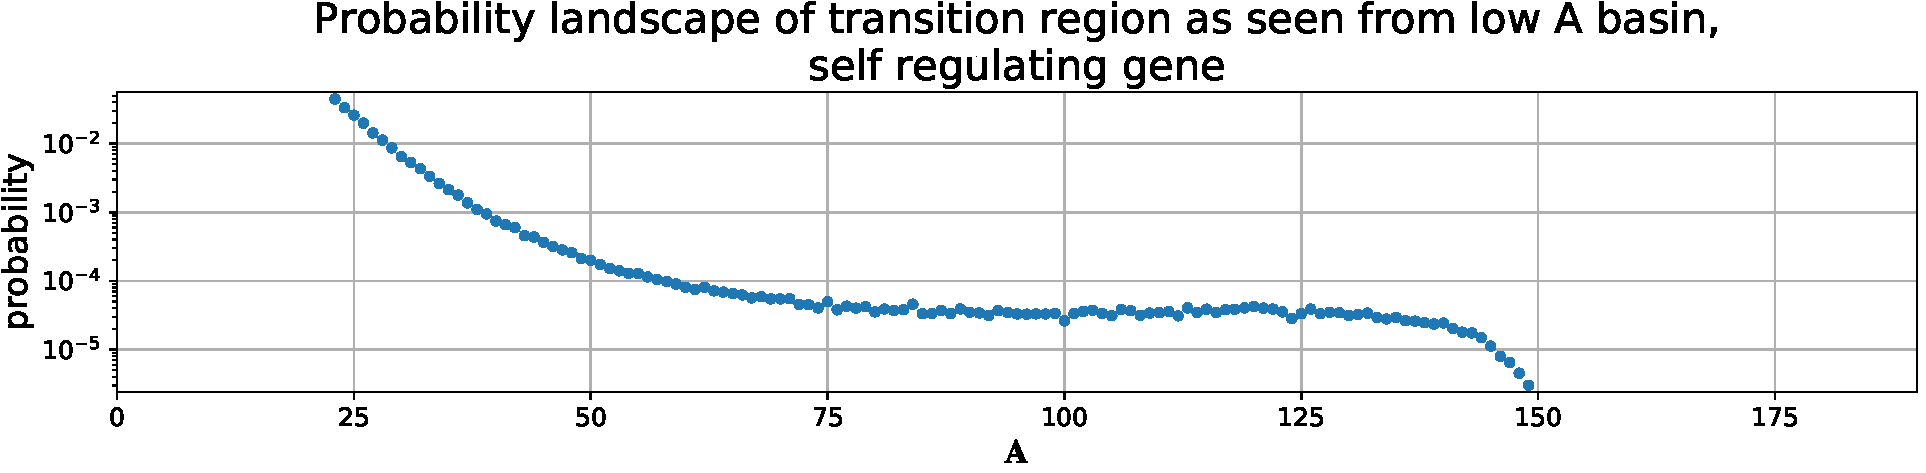
\includegraphics[width=6.0in]{{../Figures/srg_landscape_low_A_basin}.pdf}
\end{center}

\begin{center}
    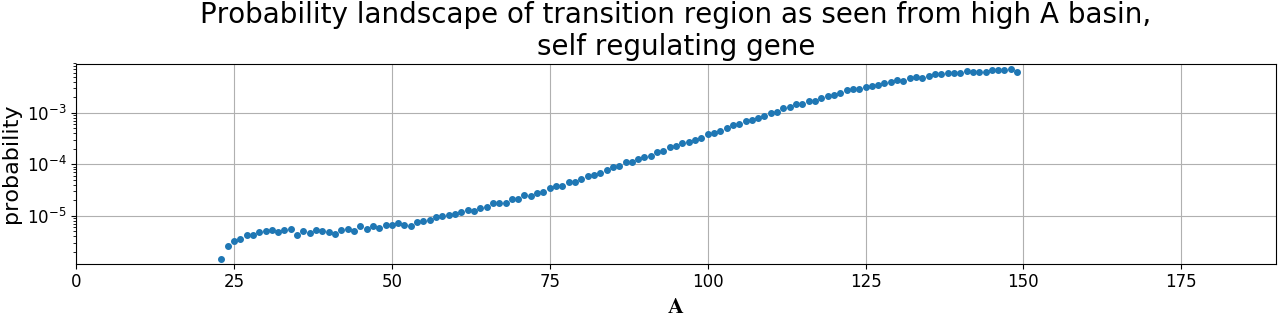
\includegraphics[width=6.0in]{{../Figures/srg_landscape_high_A_basin}.pdf}
\end{center}

\subsection{Combine the stage landscapes into the transition landscape}\label{sec:srg_transition_landscape}
Now we find the transition region landscape by taking the sum of the two stage landscapes weighted by the stage landscape factors $\stageweight$. The following script find the $\stageweight$ values and performs the combination of hists:

\inputpy{snippets/srg_landscape/transition_hist.py}

We now have an unbiased landscape of the \abr{SRG}, though for now it only spans the transition region in between the basins:

\begin{center}
    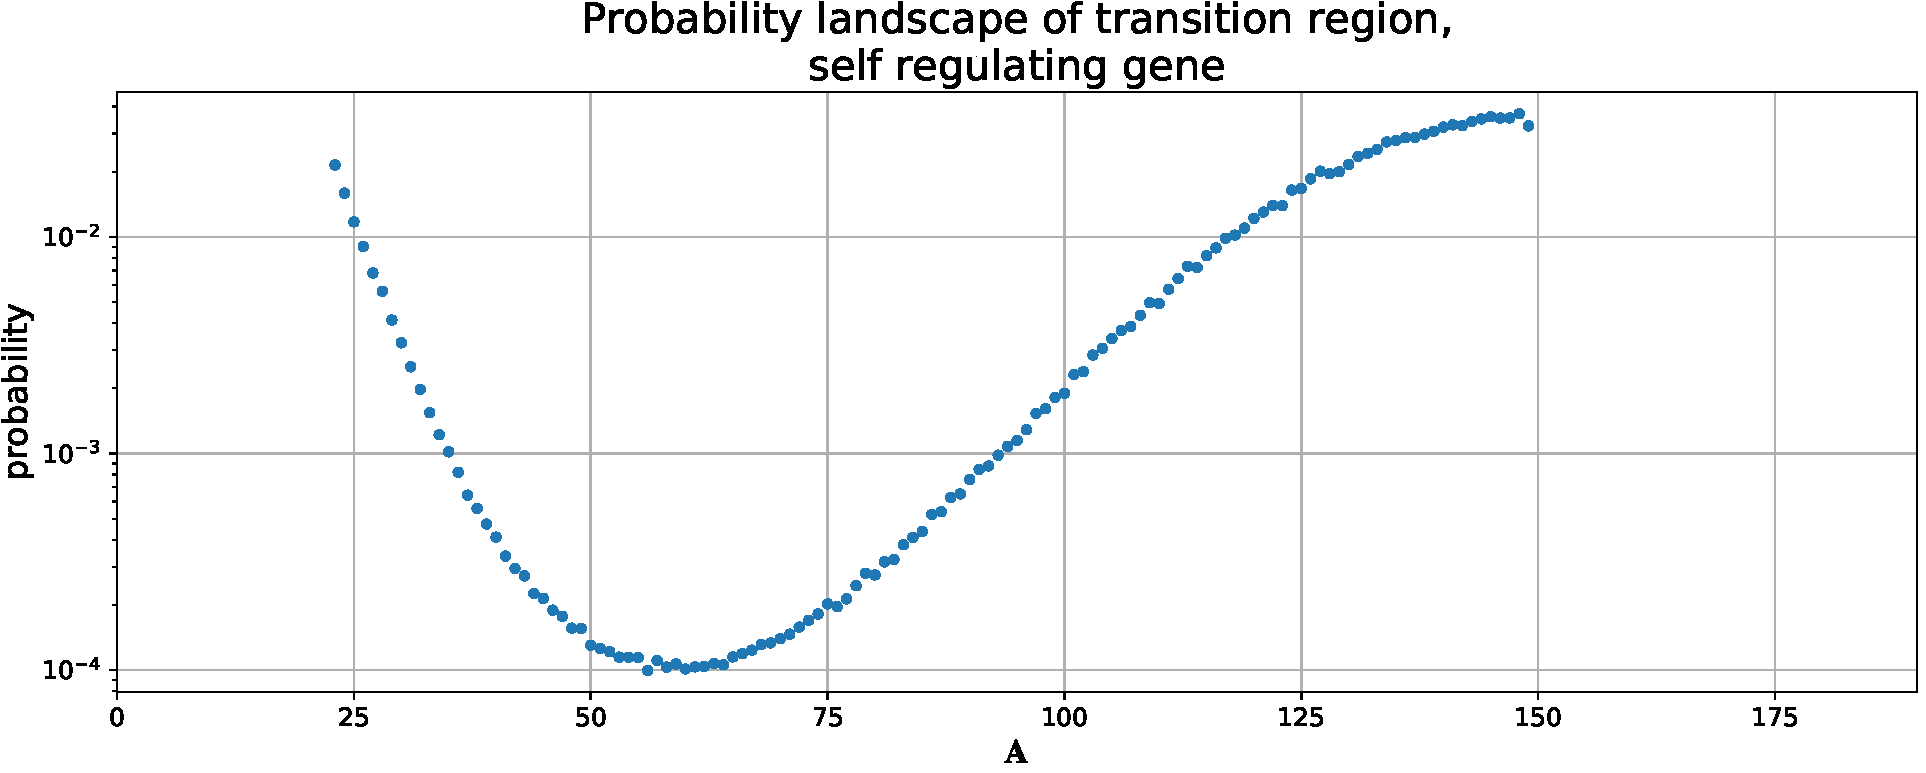
\includegraphics[width=6.0in]{{../Figures/srg_landscape_transition}.pdf}
\end{center}

\subsection{Fit together the complete landscape}\label{sec:srg_complete_landscape}

%As mentioned in \secref{sec:landscape_complete} %(see that section for math-y details)
The final step of assembling the complete landscape is also the most complicated. It proceeds in roughly 3 steps:\\
\\
\textbf{1. Sort all of the phase zero samples into two histograms}\\
One with the samples to the left of the transition minimum, and one with all of the sample to the right. The following script will accomplish this:

\inputpy{snippets/srg_landscape/split_phase_zero.py}

\textbf{2. Fit the left and right phase zero histograms onto the transition region landscape}\\
Independently, we find the weights that will smoothly fit both the left and right phase zero histograms to the transition landscape. We do this using a straightforward minimization approach, with a least-squares minimizer and a Jenson-Shannon divergence\footnote{a symmetrized form of the Kullback-Leibler divergence}. The following script will perform this fitting and report the weights:

\inputpy{snippets/srg_landscape/fit_hists.py}

\textbf{3. Patch together the phase zero histograms and the transition landscape}\\
Finally, we patch the weighted phase zero histograms together with the transition landscape in order to produce the complete landscape. The following script performs this patching:

\inputpy{snippets/srg_landscape/combine_landscape.py}

If any bin in the phase zero histograms overlaps with any bin in the transition landscape, we discard the information from the phase zero histograms in favor of that in the transition landscape, on the assumption that the transition landscape will in general be better sampled.

Now that it's all put together, the complete unbiased landscape looks like this:

\begin{center}
    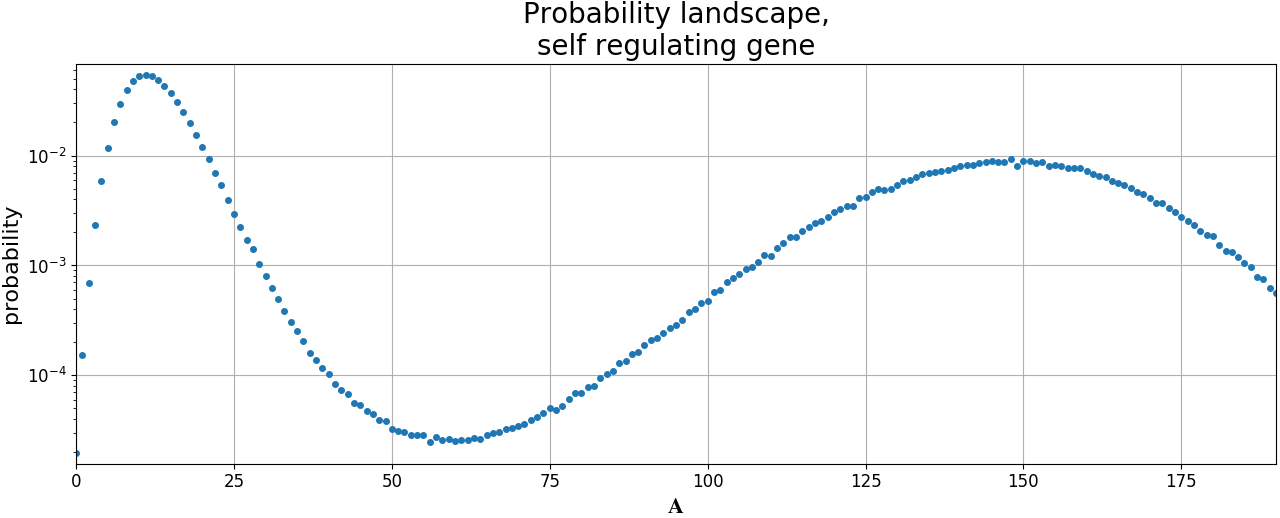
\includegraphics[width=6.0in]{{../Figures/srg_landscape}.pdf}
\end{center}

\subsection{Comparison of landscapes produced using FFPilot and direct sampling}

Shown below are a comparison of landscapes calculated using a (blue dots) 10\% error goal FFPilot simulation and (orange line) direct sampling simulation that collected $10^9$ state samples.

\begin{center}
    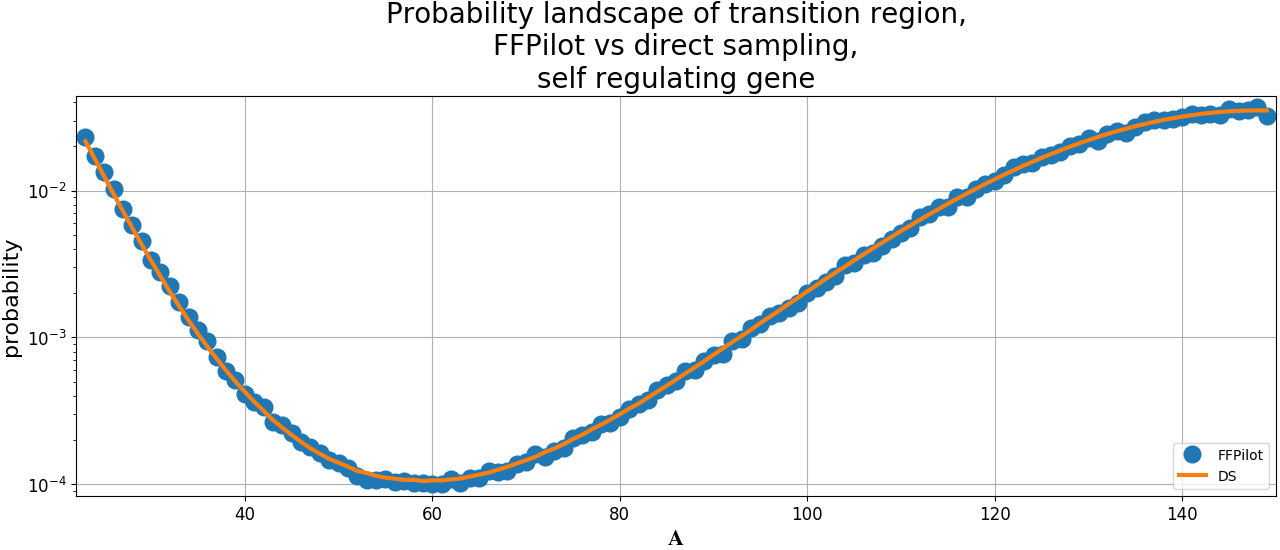
\includegraphics[width=6.0in]{{../Figures/srg_landscape_transition_ffpilot_vs_bf}.pdf}
\end{center}

\begin{center}
    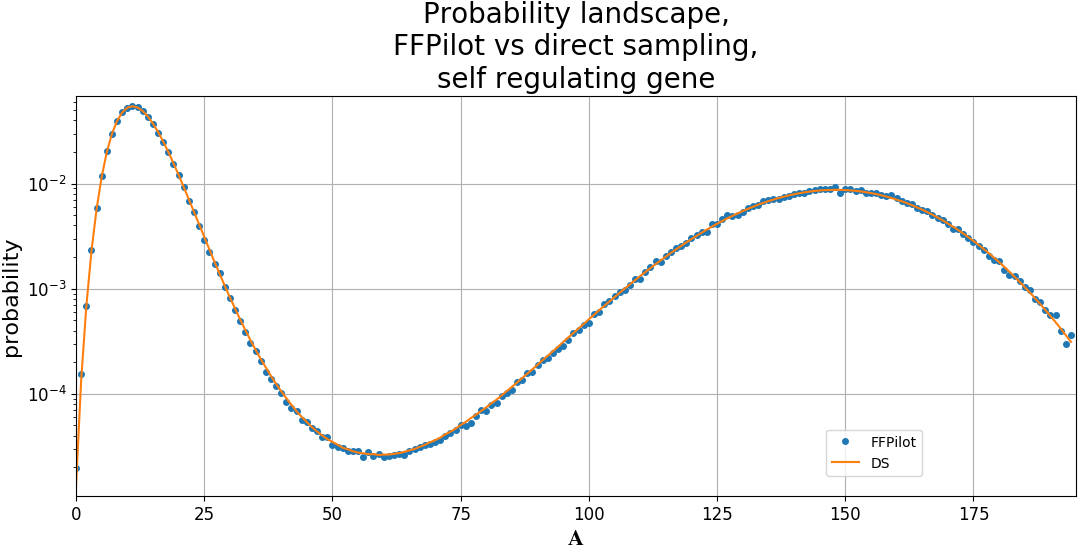
\includegraphics[width=6.0in]{{../Figures/srg_landscape_ffpilot_vs_bf}.pdf}
\end{center}

Although the FFPilot landscape is in this case slightly noisier, overall there is a high level of agreement between the FFPilot and direct sampling landscapes. This is made more impressive by the fact that, in terms of real wall-clock time, the FFPilot simulation ran to completion about 140x faster than the direct sampling one (${\sim}30$ seconds vs ${\sim}70$ minutes).
